\textbf{COLUNI 2018 -- Questão 28}\par\medskip A pele representa 15\% da massa corporal e desempenha várias funções, como proteção, regulação da temperatura corporal, sensibilidade, excreção, imunidade e ainda ativação da vitamina D. No contexto cultural, a pele, com seus diferentes tons, separa os seres humanos uns dos outros. Durante séculos a cor da pele tem servido para odiosas formas de discriminação. No entanto, com base na genética, sabemos que tal discriminação é infundada, já que biologicamente não é possível considerarmos a existência de raças entre a espécie humana. As diferenças no tom da pele estão ligadas às adaptações evolutivas dos grupos humanos aos diferentes ambientes, em função da radiação solar e da absorção da vitamina D.

% COLUNI-AUTO-FIGURES-BEGIN
\begin{figure}[htbp]
\centering
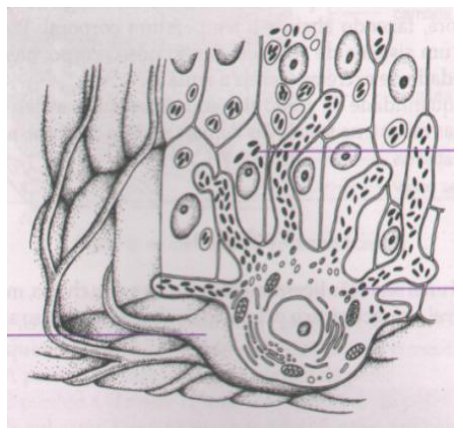
\includegraphics[width=0.95\linewidth]{static/simulados/coluni/figuras/2018/questao-28/figura-1.png}
\end{figure}
% COLUNI-AUTO-FIGURES-END

Fonte: TELECURSO 2000 2º Grau. \textbf{Biologia}. Vol. 2. São Paulo: Ed. Globo, 2002. p. 104.

\par

Com base no texto e na análise da figura, é CORRETO afirmar que a cor da pele é apenas uma característica humana que depende, principalmente, da quantidade de:


\begin{enumerate}
\item melatonina, produzida pelas células epiteliais da epiderme e presente nas células da derme.
\item melanina, produzida pelas células epiteliais da epiderme e presente nas células da derme.
\item melatonina, produzida pelos melanócitos e presente nas células epiteliais da epiderme.
\item melanina, produzida pelos melanócitos e presente nas células epiteliais da epiderme.\end{enumerate}
